\documentclass[12pt]{article}
\usepackage[a4paper,left=27mm,right=27mm,top=24mm,bottom=22mm]{geometry}
\usepackage[space]{ctex}
\usepackage{graphicx}
\usepackage{float}
\usepackage{subfigure}
\usepackage{amsmath}
\usepackage{amsfonts,amssymb}
\title{\LARGE\textbf{Grabcut}}
\author{SA21010060 周俊亦}
\date{}

\begin{document}
	\maketitle
	\renewcommand{\abstractname}{Abstract}
	\begin{abstract}
		静止图像中高效的交互式前景/背景分割问题在图像编辑中具有重要的实际意义。Grabcut是一种著名的图像分割算法,该算法将图像理解成图,基于高斯混合模型与图的最大流最小割算法对图片进行前景/背景提取。本报告对"Grabcut"论文中提到的算法进行复现。
	\end{abstract}
	
	\section{概述}
	Grabcut是一种实现前景后景分离的算法。该算法将图像看成有向图,应用高斯混合模型与最大流最小割定理对图像进行处理。以下将对算法原理进行介绍。
	
	
	
	\section{高斯混合模型GMM(Gaussian Mixed Model)}
	高斯混合模型(Gaussian Mixed Model)指多个高斯分布函数的线性组合,理论上GMM可以拟合出任意类型的分布,通常用于解决同一集合下的数据包含多个不同的分布的情况.
	
	设有随机变量 $\boldsymbol{X}$,则混合高斯模型可以用下式表示:
	
	$$
	p(\boldsymbol{x})=\sum_{k=1}^{K} \pi_{k} \mathcal{N}\left(\boldsymbol{x} \mid \boldsymbol{\mu}_{k}, \boldsymbol{\Sigma}_{k}\right)
	$$
	
	其中 $K$ 为分量总数, $\mathcal{N}\left(\boldsymbol{x} \mid \boldsymbol{\mu}_{k}, \boldsymbol{\Sigma}_{k}\right)$,为混合模型中的第 $k$ 个分量,$\pi_{k}$ 是混合系数,满足:
	
	$$
	\begin{aligned}
		&\sum_{k=1}^{K} \pi_{k}=1 \\
		&0 \leq \pi_{k} \leq 1
	\end{aligned}
	$$
	
	实际上,可以认为 $\pi_{k}$ 是每个分量 $\mathcal{N}\left(\boldsymbol{x} \mid \boldsymbol{\mu}_{k}, \boldsymbol{\Sigma}_{k}\right)$ 的权重。
	
	通过极大似然估计法,可以对 GMM 进行参数估计。Grabcut对图像 RGB 三通道的高斯混合模型 GMM 进行参数估计。
	
	
	\section{最大流最小割定理}
	
	最大流最小割定理:一个网中所有流中的最大值等于所有割中的最小容量。即在任何网络中,最大流的值等于最小割的容量。\\
	
	
	直觉解释:最小割是从源点到汇点的网络流的必经之路,最大流也是网络流,不可能大于路的容量,即最大流不可能大于最小割的容量;如果最大流小于最小割,说明最小割有容量空余,边的容量没有物尽其用,必然可以加大流量,因此,最大流不可能小于最小割。
	
	
	\section{Grab Cut}
	算法步骤如下:
	
	\begin{enumerate}
		\item [1.] 用户定义矩形区域,矩形外的区域被自动认为是背景,在矩形区域内部,可用背景中的数据来区分它里面的前景和背景区域
		\item [2.] 用高斯混合模型(GMM)来对背景和前景建模,并用极大似然估计法估计模型参数
		
		$$
		k_{n}:=\arg \min _{k_{n}} D_{n}\left(\alpha_{n}, k_{n}, \theta, z_{n}\right)
		$$
		
		$$
		\underline{\theta}:=\arg \min _{\underline{\theta}} U(\underline{\alpha}, \mathbf{k}, \underline{\theta}, \mathbf{z})
		$$
		
		\item [3.] 将图像中的每一个像素看做通过虚拟边与周围像素相连接,每条边都有一个属于前景或者背景的概率,这是基于它与周边像素颜色上的相似性
		\item [4.] 前景看成源节点,背景看成终端节点,用最大流最小割算法进行前景后景分离
		
		$$
		\min _{\left\{\alpha_{n}: n \in T_{U}\right\}} \min _{\mathbf{k}} \mathbf{E}(\underline{\alpha}, \mathbf{k}, \underline{\theta}, \mathbf{z}) .
		$$
		
	\end{enumerate}
	
	
	
	
	\section{实验分析}
	实验使用 Qt5.12.2 与 OpenCV3.4.15 进行算法验证,使用 gcc 编译生成。
	
		\subsection{程序界面}
	\begin{figure}[H]
		\centering
		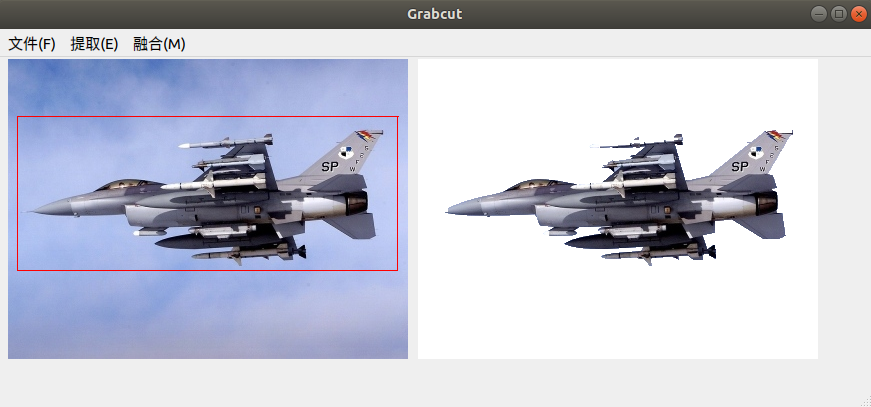
\includegraphics[width=6in]{./ui.png}
		\centering
		\caption{程序界面}
	\end{figure}
	
	用户可以使用矩形框框选图像,且可交互指定前景背景区域,提取前景或者背景,并可以替换背景图片。
	
	\subsection{Examples}
	
	\subsubsection{矩形框选}
	
	\begin{figure}[H]
		\centering
		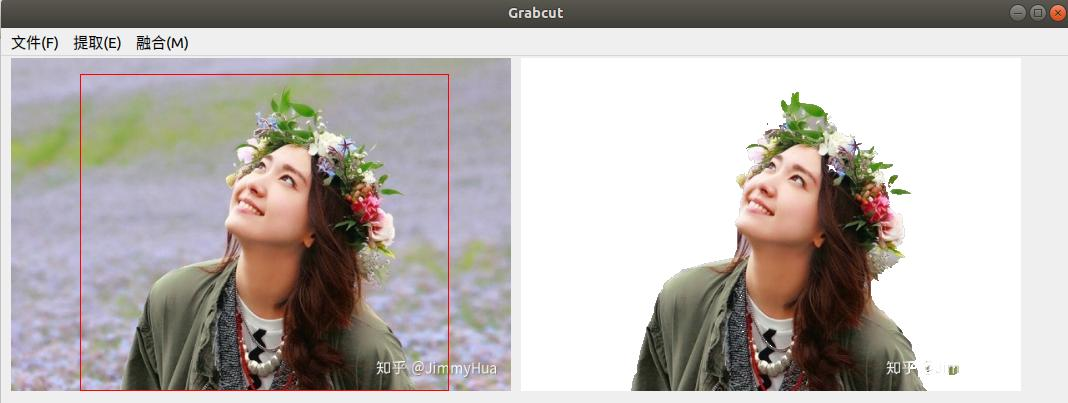
\includegraphics[width=6in]{./1.png}
		\centering
		\caption{矩形框选}
	\end{figure}
	图例展示了直接矩形框选效果,有些许瑕疵。
	
	\subsubsection{交互框选}
	
	\begin{figure}[H]
		\centering
		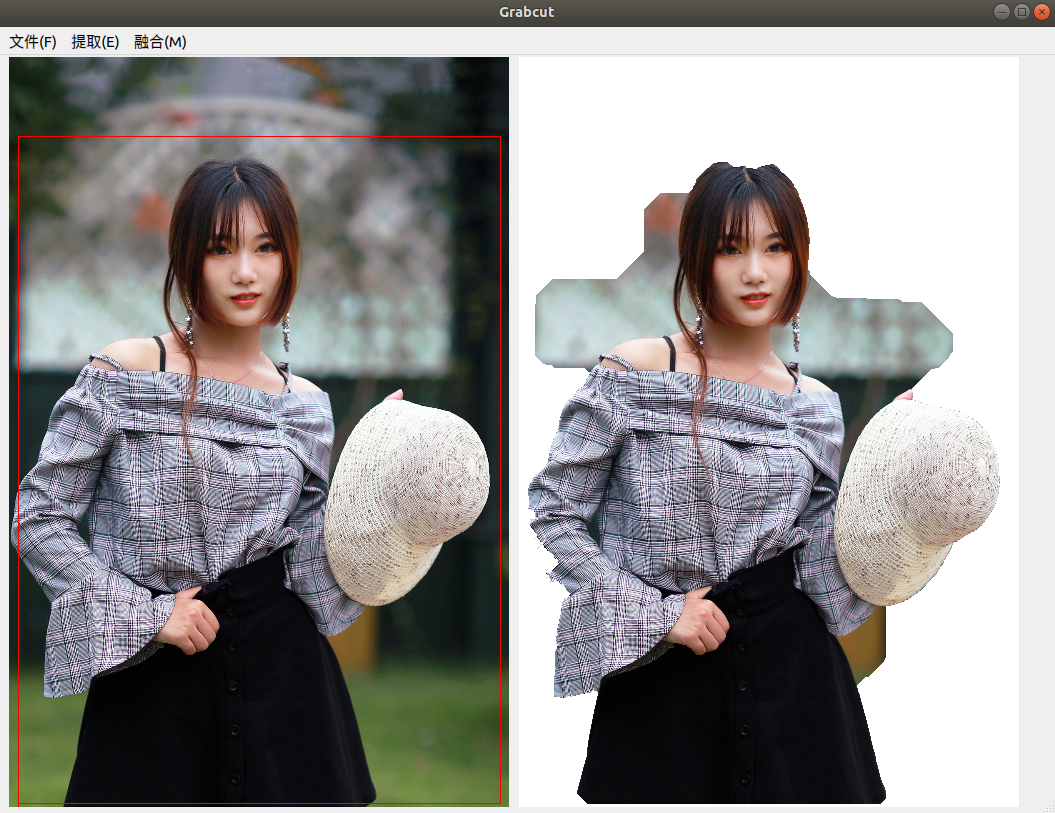
\includegraphics[width=5in]{./2_1.png}
		\centering
		\caption{矩形框选}
	\end{figure}
	上图展示了直接矩形框选效果,可以发现人物过滤并不完整,效果很差。
	
	\begin{figure}[H]
		\centering
		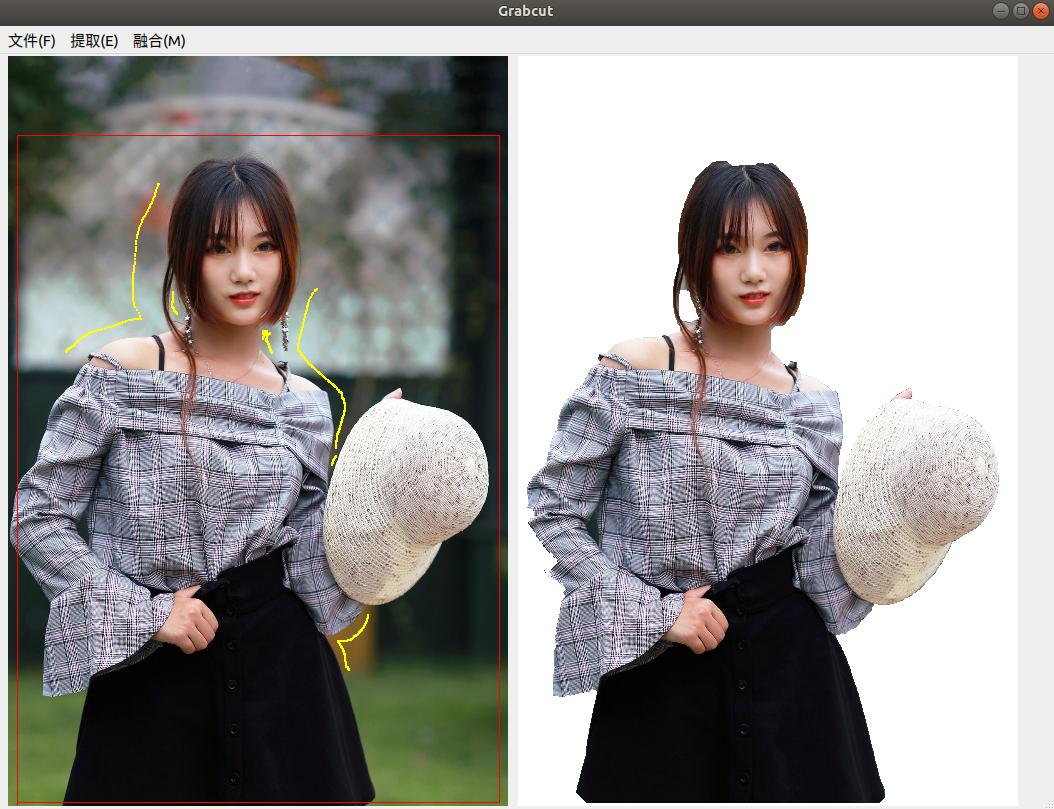
\includegraphics[width=5in]{./2_2.png}
		\centering
		\caption{设定背景框选}
	\end{figure}
	交互指定背景后如上图,整体效果显然好了不少,\textbf{但人物左侧肘关节的衣袖不全,头顶头发部分不全,且右侧耳环信息被抹去}。
	
	\begin{figure}[H]
		\centering
		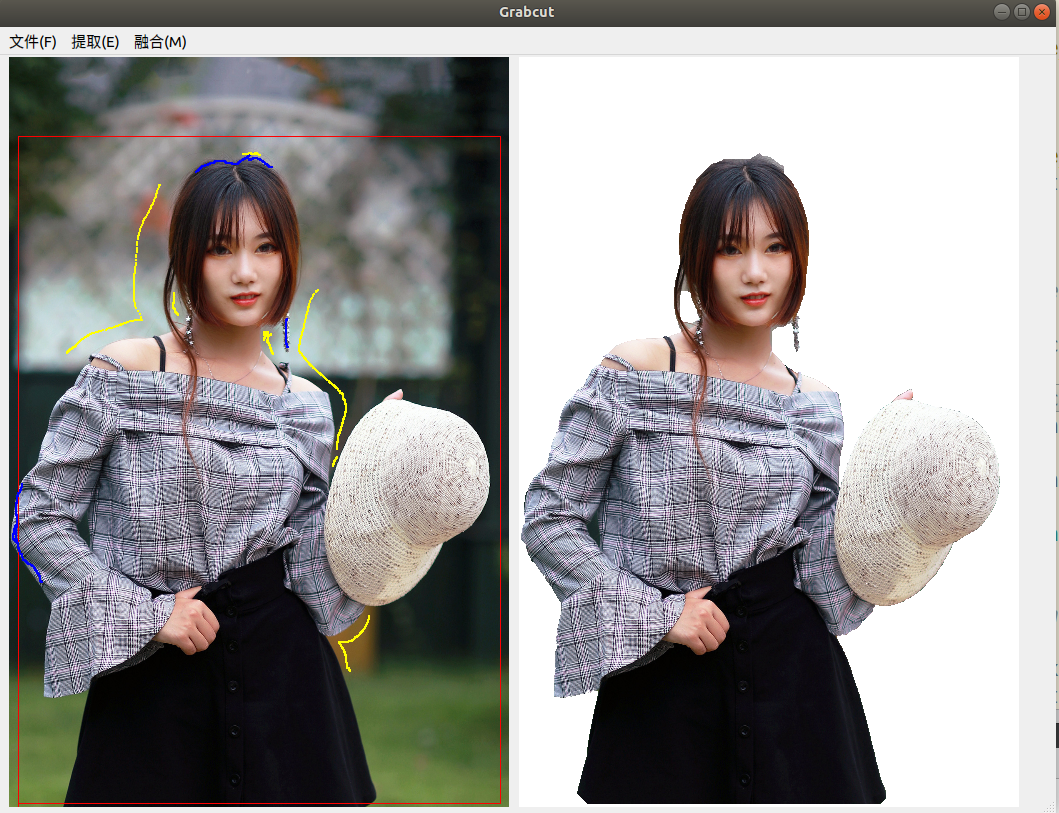
\includegraphics[width=5in]{./2_3.png}
		\centering
		\caption{设定背景框选}
	\end{figure}
	继续增加指定前景后如图(蓝色线为指定前景),补全了头发部分、衣袖部分、以及耳环部分,整体效果良好。
	
	\subsubsection{背景融合}
	
	\begin{figure}[H]
		\centering
		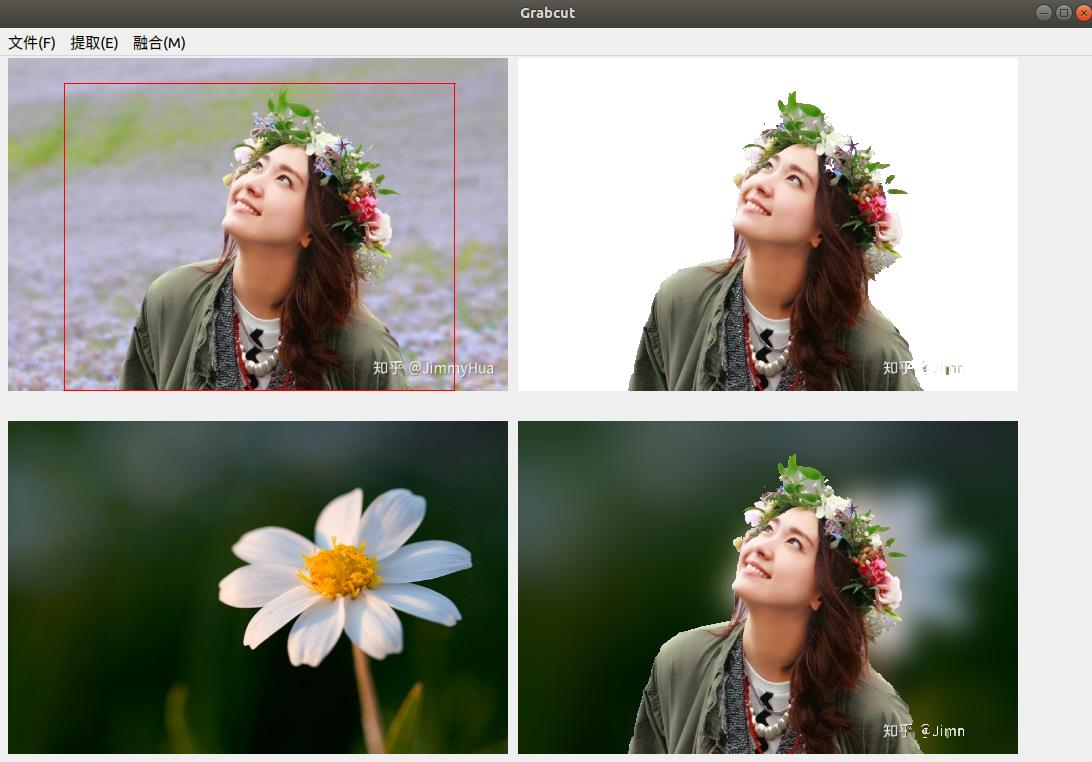
\includegraphics[width=4in]{./3.png}
		\centering
		\caption{背景融合}
	\end{figure}
	如图展示背景融合结果,将分离的前景与高斯模糊后的背景叠加,达到更改背景效果。
	
	
	\section{实验总结}
	以前没有了解过图论的知识,通过这次实验,对图的最大流最小割问题有了一定的了解。
	
	在实验中发现,当背景颜色与前景相近时,算法无法较好的分割前景后景,这是算法原理所必然导致的结果,此时需要精确的人工交互前后景划分。
	
	附睿客网代码链接:
	
	链接:https://rec.ustc.edu.cn/share/78a3e1a0-510f-11ec-be2b-d9ecaf068bd0
	
	\begin{thebibliography}{99}
	
		[1]Carsten Rother, Vladimir Kolmogorov, and Andrew Blake. 2004. "GrabCut": interactive foreground extraction using iterated graph cuts. ACM Trans. Graph. 23, 3 (August 2004), 309–314. DOI:https://doi.org/10.1145/1015706.1015720
		
	\end{thebibliography}
\end{document}

